% GENERATED by latex/convert.py -- see body.tex.
\begin{figure}[htbp]
\centering
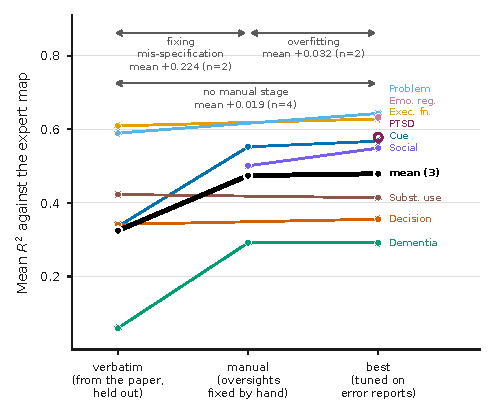
\includegraphics[width=\linewidth]{../../reports/nature_methods_figures/figureS1_tier_progression.pdf}
\caption{\textbf{Recovery of reference maps is sensitive to criteria specification.} Project-level mean spatial correspondence (\emph{r}\textsuperscript{2}) across three configurations: criteria closely transcribed from the published methods (`verbatim'), criteria manually corrected for identified oversights (`manual'), and configurations selected after further LLM-assisted refinement using benchmark feedback (`best'). Paired comparisons between distinct evaluated configurations showed a mean increase of +0.221 after manual correction (\emph{n} = 2 projects: dementia and cue reactivity) and +0.031 after subsequent refinement (\emph{n} = 2 projects: cue reactivity and social cognition). Projects with no manual correction, saw a small improvement of +0.018 between verbatim and best configurations (\emph{n} = 4)}
\label{fig:tiers}
\end{figure}

\begin{figure}[htbp]
\centering
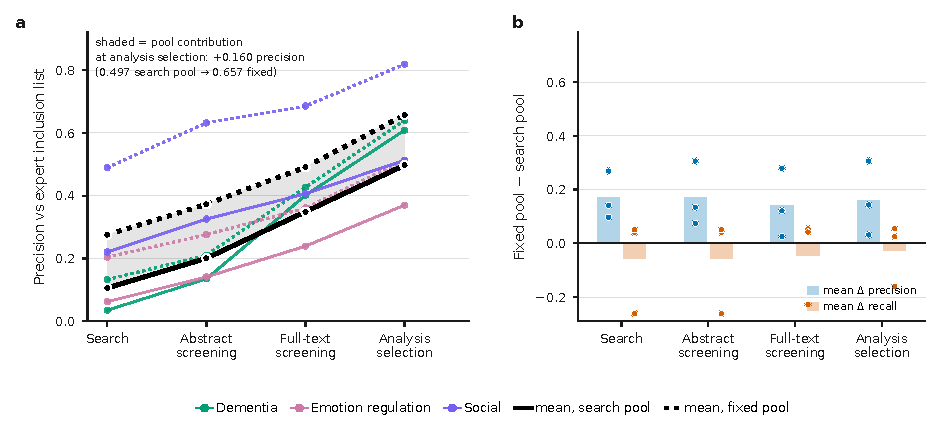
\includegraphics[width=\linewidth]{../../reports/nature_methods_figures/figureS2_pool_mismatch.pdf}
\caption{\textbf{Candidate article pools influence measured screening precision.} Precision against expert inclusion lists when the same eligibility criteria are applied to articles retrieved by AutoNIMA's PubMed searches (solid lines) or candidate screening lists obtained from the original reviewers (dotted lines). Author-provided lists were available for three projects: dementia, emotion regulation and social cognition. At the final stage, articles are retained if at least one analysis is selected for a target contrast. Mean final precision increased from 49.7\% to 65.7\% when author-provided lists were used, a difference of 16 percentage points. This comparison indicates that differences between the candidate pools considered by automated and original reviewers can lower apparent precision against published inclusion lists. Recall decreased in one project because the author-provided list covered only a subset of the originally screened articles; the remaining screening records were unavailable.}
\label{fig:pools}
\end{figure}

\begin{figure}[htbp]
\centering
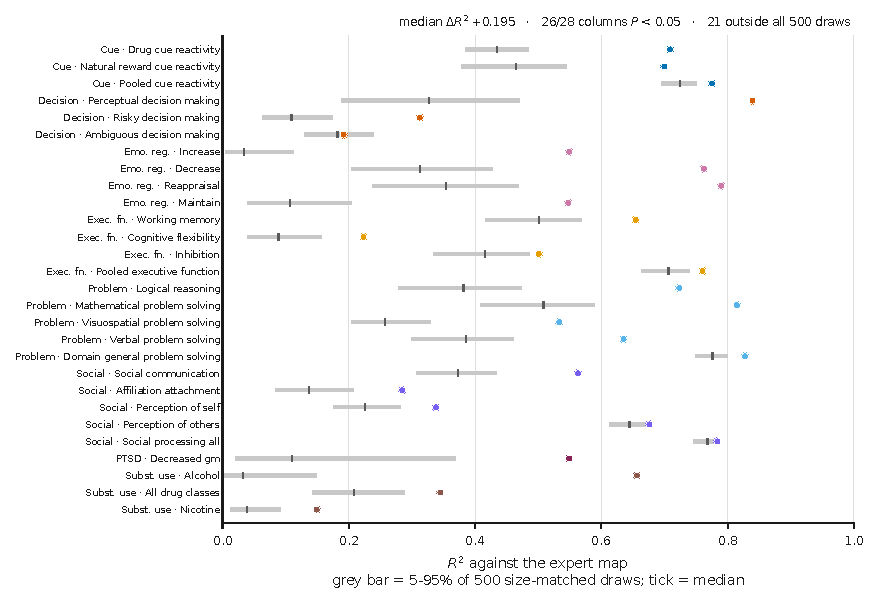
\includegraphics[width=\linewidth]{../../reports/nature_methods_figures/figureS3_size_matched_null.pdf}
\caption{\textbf{Analysis-level selection improves map recovery relative to equally sized random subsets.} Observed correspondence with reference maps (\emph{r}\textsuperscript{2}) compared with the mean and 5th--95th percentile range of a random-selection distribution for each of 28 target contrasts. For each contrast, 500 subsets were sampled from the same candidate analysis pool, each containing the same number of analyses as the selected set. MKDA was repeated for every subset using the same settings as the observed synthesis. This comparison controls the number of pooled analyses while varying which analyses are included. The median improvement over the mean random-selection result was $\Delta$r\textsuperscript{2} = +0.188. Observed correspondence exceeded the random-selection distribution at an unadjusted, per-contrast threshold of P \textless{} 0.05 in 26 of 28 contrasts, one of them marginally (P = 0.0499). Empirical \emph{P} values were calculated as one plus the number of random subsets achieving at least the observed correspondence, divided by 501. Percentile ranges describe variation across random subsets and are not confidence intervals for the observed result.}
\label{fig:null}
\end{figure}

\begin{figure}[htbp]
\centering
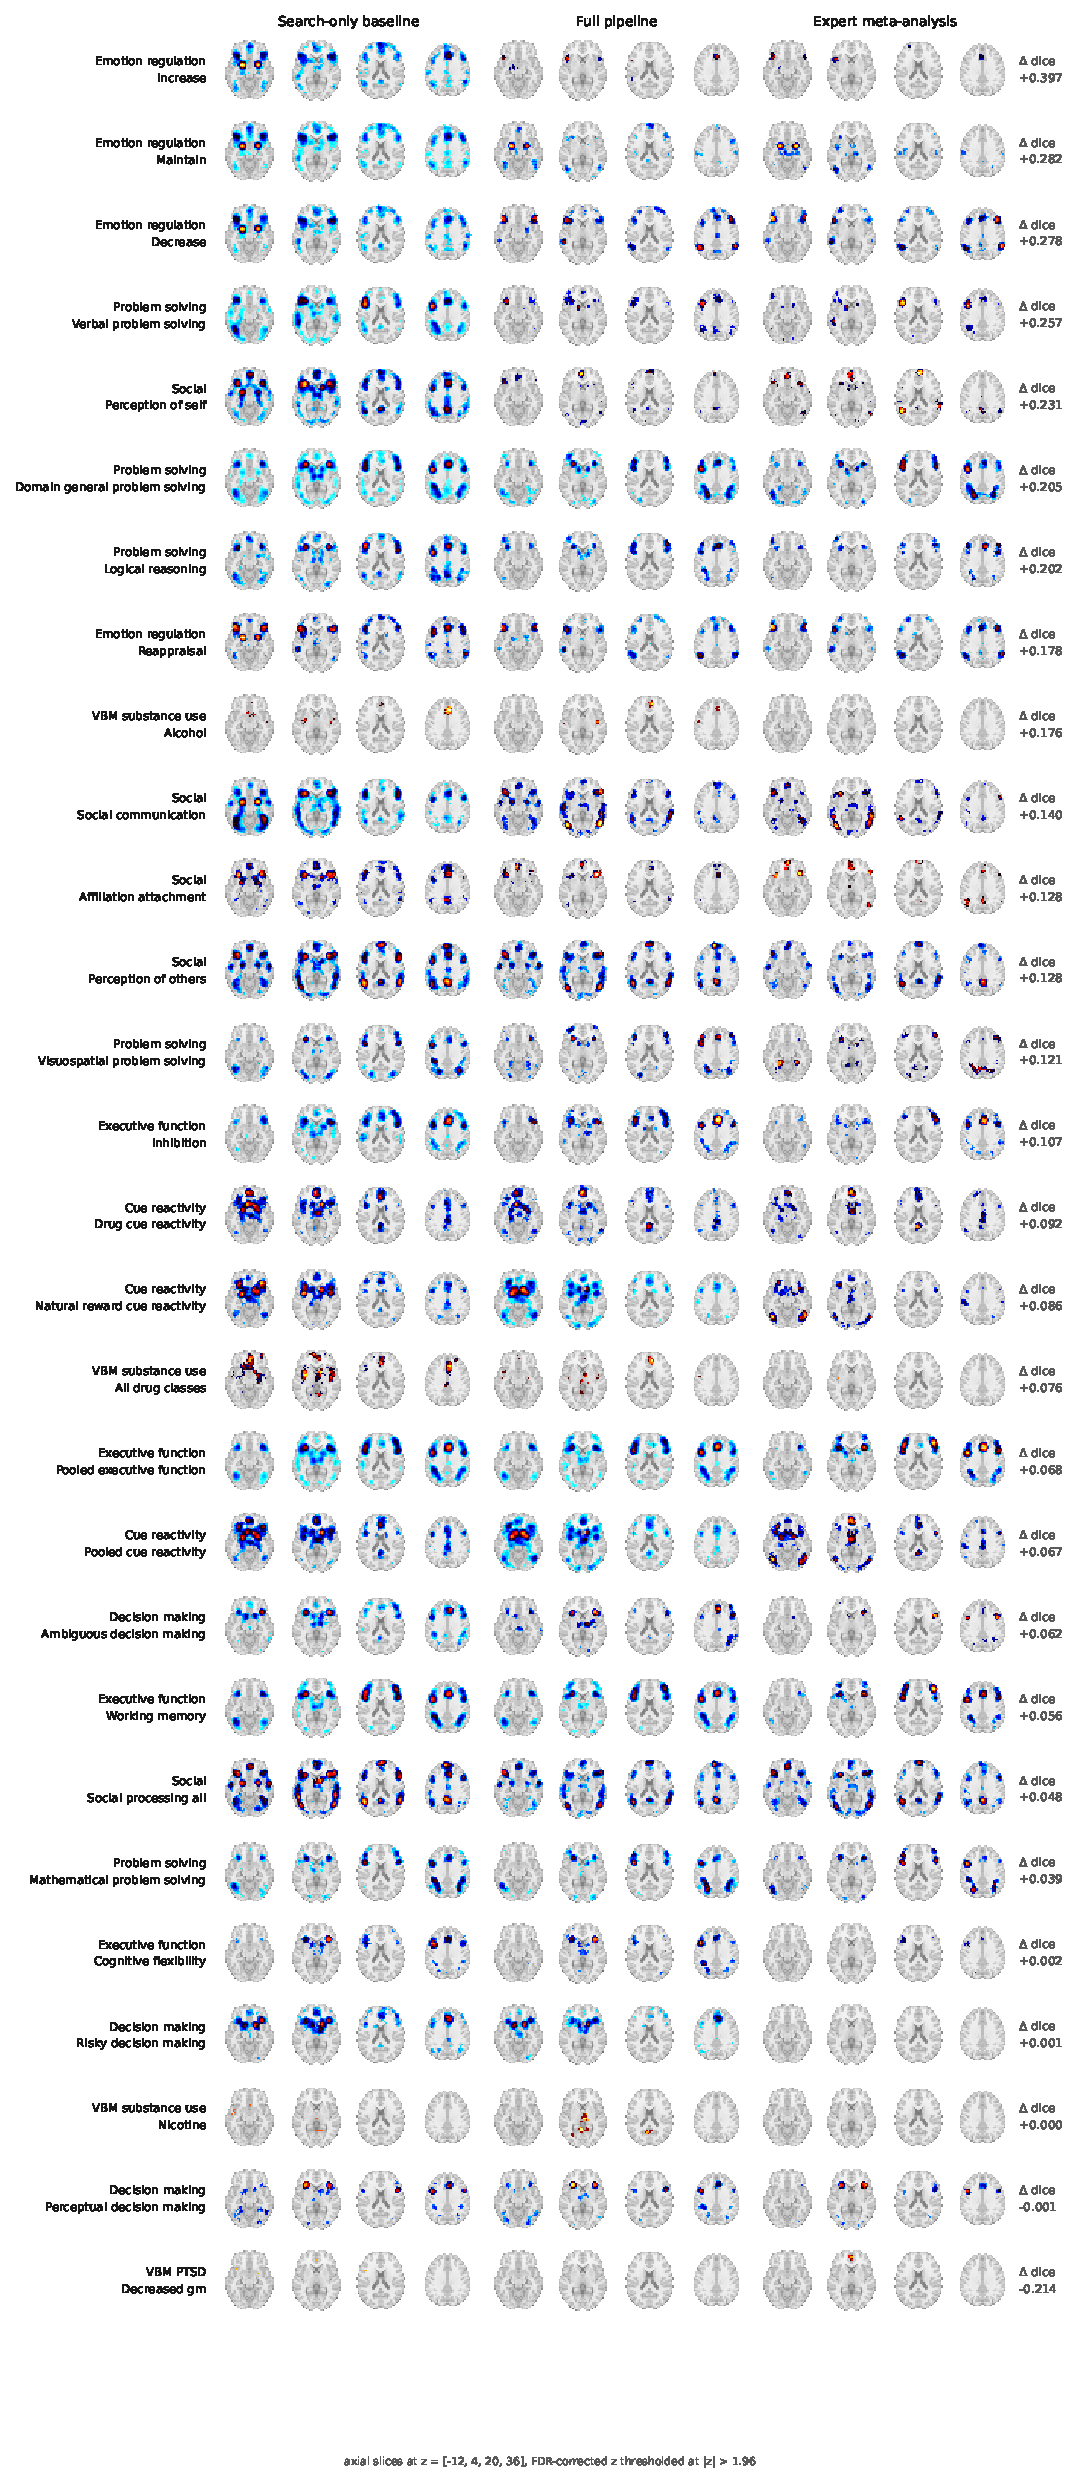
\includegraphics[height=0.92\textheight,keepaspectratio]{../../reports/nature_methods_figures/figureS4_brain_maps_all.pdf}
\caption{\textbf{Reference, search-only and AutoNIMA maps across all evaluated contrasts.} Axial slices at four levels show the expert reference, search-only baseline and AutoNIMA map for each of the 28 target contrasts included in Fig.~\ref{fig:correspondence}. Maps are displayed at \emph{z} \textgreater{} 1.96, the threshold used for the reported overlap analyses. Squared voxelwise correlations were calculated from unthresholded maps. All evaluated contrasts are shown, including those with small improvements or lower correspondence after automated curation.}
\label{fig:maps}
\end{figure}

\begin{figure}[htbp]
\centering
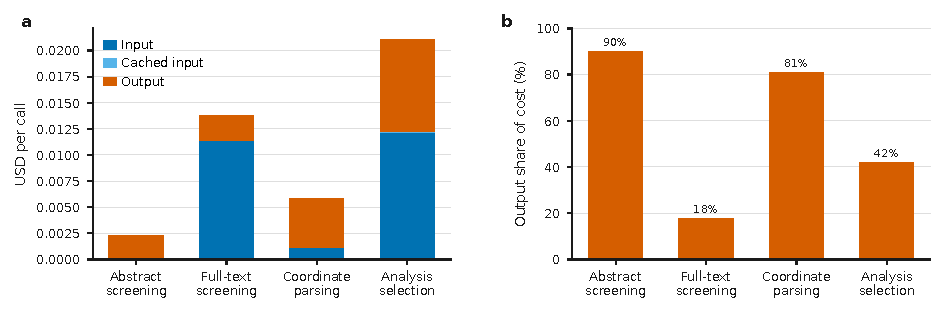
\includegraphics[width=\linewidth]{../../reports/nature_methods_figures/figureS5_measured_cost.pdf}
\caption{\textbf{Model-use costs estimated from recorded token consumption.} Mean cost per LLM call at each workflow stage, separated into uncached input, cached input and output token charges. Costs were calculated from recorded token consumption and the applicable token prices (Methods). Mean per-call costs were US\$0.0023 for abstract screening, US\$0.0138 for full-text screening, US\$0.0059 for coordinate parsing and US\$0.0211 for analysis selection. Output tokens accounted for most of the abstract-screening cost. Applying measured usage rates to the observed number of operations at each stage gave an estimated mean cost of US\$21.55 per project and approximately US\$194 across all nine projects. The median project-level cost per study contributing to a final map was US\$0.085. Project totals account for differences in the number of articles reaching each stage. These estimates cover model use and exclude article-access charges, other computing costs and researcher time.}
\label{fig:cost}
\end{figure}
